% !TEX root = ../my-thesis.tex
%

\chapter{Contexte scientifique}
\label{sec:contexte}
%\cleanchapterquote{Un petit chapitre pour le doctorant, un grand chapitre pour l'humanité}{Doctorant anonyme}{(Citation temporaire)}
\newV{Le fil conducteur de cette thèse est délimité par deux contextes : tout d'abord un contexte clinique correspondant aux besoins des médecins en termes de segmentation des vaisseaux du foie ; ensuite un contexte technique dont les problématiques sont dictées par les méthodes d'acquisition d'images et la quantité de données exploitables.} Dans ce chapitre, nous décrivons le foie et ses particularités anatomiques. Nous présentons ensuite les modalités d'imagerie courantes pour cet organe : l'imagerie par résonance magnétique et la tomodensitométrie par rayons X. Nous présentons ensuite les avantages et les contraintes liés à ces modalités avant de présenter un tour d'horizon des principales bases de données publiques disponibles.
\section{Contexte clinique}
\label{sec:contexte:clinique}
Le foie est un organe vital pour le fonctionnement du corps humain. Il est impliqué dans de nombreux systèmes vitaux : contrôle de la glycémie, élimination des toxines du sang, participation à la digestion et au système immunitaire. Le suivi des dysfonctionnements de cet organe est donc crucial pour les médecins. Le foie est situé au niveau de l'abdomen, au-dessous des poumons. Il est adjacent à l'estomac et au cœur (Fig. \ref{fig:liver}).

\newV{Dans un système vasculaire classique, le sang oxygéné est distribué dans l'organe par les artères. Il passe ensuite à travers un réseau de capillaires, de très fins vaisseaux, au niveau desquels s'effectuent les échanges entre les cellules de l'organe et le sang. Le sang appauvri en oxygène est ensuite renvoyé vers le cœur par le système veineux. Au niveau du foie, ce circuit d'oxygénation est formé par les vaisseaux issus de l'artère hépatique et les veines hépatiques, elles-mêmes connectées à la veine cave inférieure. La particularité du foie est qu'il est alimenté par un second système veineux qui connecte le foie à trois organes : l'estomac, le pancréas et la rate. C'est par la veine porte que ce système veineux alimente le foie en nutriments.}
\begin{figure}[!ht]
    \centering
    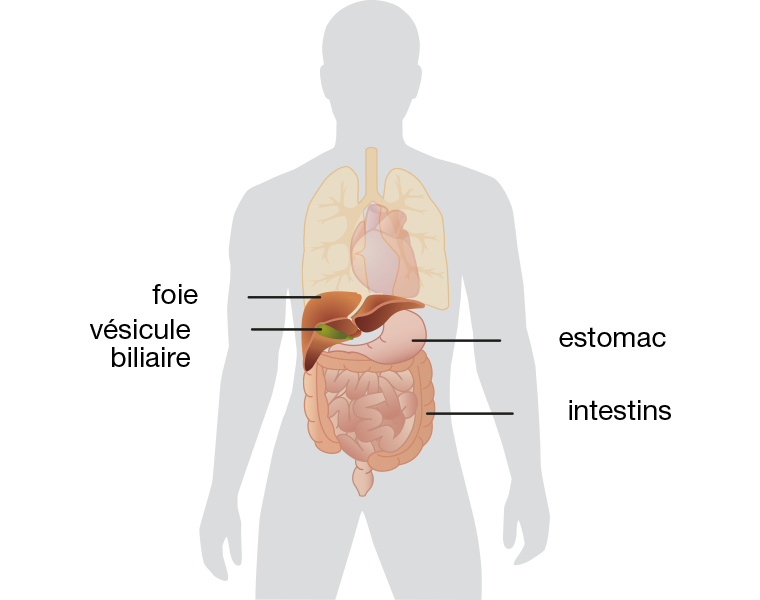
\includegraphics[height=8cm]{Images/Liver.png}
    \caption[Hello world]{Positionnement du foie chez l'homme. Il se situe sous les poumons. Il est proche du cœur et adjacent à l'estomac.\protect \footnotemark}
    \label{fig:liver}
  \end{figure}

La veine cave est connectée au foie par sa partie supérieure alors que la veine porte entre dans le foie par son centre via le tronc porte (Fig. \ref{fig:liver veins}). Le tronc porte se divise une première fois à l'entrée du foie pour former les veines  porte droite et gauche. Ces deux branches se subdivisent ensuite à plusieurs reprises afin d'alimenter l'ensemble des tissus du foie.

Un intérêt particulier est porté à la veine porte puisque ses ramifications forment six régions du foie indépendamment approvisionnées les unes des autres. Cette cartographie, illustrée en figure \ref{fig:liver veins} est largement adoptée par les médecins sous le nom de segmentation de Couinaud. Cette segmentation est notamment utilisée lors de la planification d'opérations d'extraction de tumeurs pour définir les limites des zones à extraire. \footnotetext{Source : \url{https://www.chuv.ch/fr/transplantation/cto-home/patients-et-familles/foie}}
\begin{figure}[!ht]
    \centering
    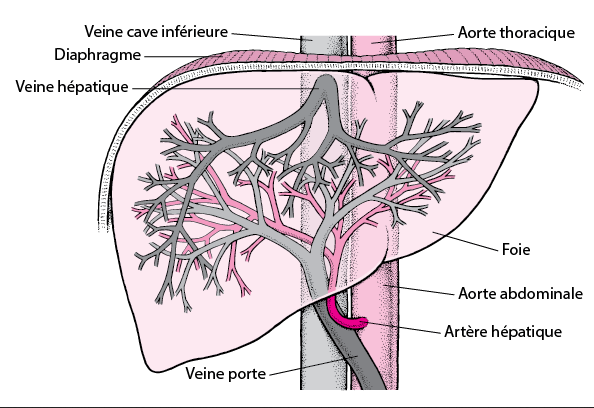
\includegraphics[width=0.4\textwidth]{Images/Liver_vasculature.png}
    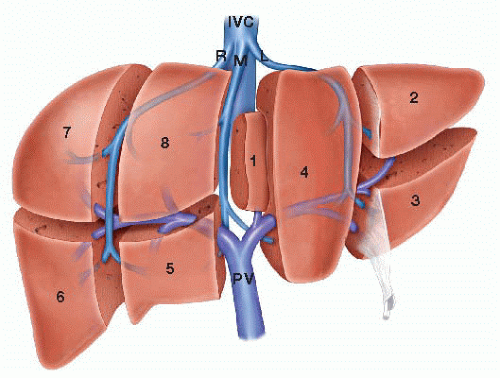
\includegraphics[width=0.4\textwidth]{Images/Couinaud.png}
    \caption{À gauche, le système vasculaire du foie et ses principaux réseaux vasculaires : veine hépatique, veine porte, artère hépatique. À droite, la segmentation de Couinaud dont chaque segment est alimenté par une branche de la veine porte.\protect \footnotemark} 
    \label{fig:liver veins}
  \end{figure}
  \footnotetext{Système veineux : \url{https://www.merckmanuals.com/fr-ca/accueil/troubles-du-foie-et-de-la-v\%C3\%A9sicule-biliaire/maladies-vasculaires-du-foie/pr\%C3\%A9sentation-des-maladies-vasculaires-du-foie} }
  \footnotetext{Schéma de Couinaud : \url{https://basicmedicalkey.com/surgical-anatomy-of-the-liver/}}

La hiérarchie des embranchements des systèmes veineux et artériel est relativement stable dans la population, mais des variations entre les individus peuvent survenir. Une étude, réalisée par Fang et al. \cite{Fang2012_Liver_vein_variations} effectuée sur 200 patients, montre que le schéma "classique" ne représente que 61 \percent{}des cas. Les 39 \percent{}restants se divisent en divers cas particuliers. Le réseau lymphatique est aussi présent au niveau du foie, mais son faible diamètre par rapport à la résolution TDM et IRM rend ce système invisible sur la plupart des imageries hépatiques. 

\newV{Outre les systèmes vasculaires et lymphatiques, le foie est entièrement composé de petits groupes de cellules nommées hépatocytes qui lui donnent un aspect homogène lorsqu'il est sain. Lorsqu'il est atteint de cirrhose, l'aspect du foie change et devient fibreux. Si la cirrhose évolue en cancer du foie (hépatocarcinome), des tumeurs visibles sous la forme de zones de densités différentes sont observables à l'imagerie. Selon la sévérité de la maladie, le foie peut changer drastiquement d'aspect (Fig. \ref{fig:unhealthy liver}) et se contracter, écrasant ainsi les systèmes vasculaires. Une partie des vaisseaux peut donc changer d'aspect ou disparaitre des images acquises. }
\begin{figure}
    \centering
    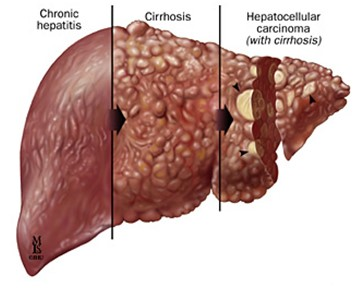
\includegraphics[height=6cm]{Images/Liver_cirrhosis_stages.jpg}
    \caption{Différents stades de maladie du foie. L'hépatite chronique (gauche) peut évoluer en cirrhose (centre) et se transformer en cancer du foie (droite)\protect \footnotemark.}
    \label{fig:unhealthy liver}
\end{figure}

La plupart des images de foie sont des images de foies malades dans la mesure où les actes médicaux ne sont pas réalisés sans suspicion de maladie.
\footnotetext{Source : \url{https://www.addictaide.fr/alcool-la-cirrhose-du-foie-est-elle-une-maladie-microbienne/}}
\section{Contexte d'imagerie}
\label{sec:contexte:images}
Les avancées technologiques dans l'imagerie médicale sont motivées par le besoin de connaitre le corps du patient tout en limitant les opérations intrusives. Des techniques permettant d'obtenir une image d'une partie interne du corps ou d'un organe ont donc vu le jour. On peut par exemple citer l'imagerie par ultrasons qui permet d'obtenir une image en envoyant des ondes sonores à travers un medium. Le calcul du temps de propagation permet ensuite de générer une image en fonction de la densité des tissus traversés. On peut aussi citer la plaque radiographique, qui permet de créer une image en deux dimensions en exposant une plaque sensible aux rayonnements à une source de photons. En plaçant le corps entre la plaque et la source, les tissus absorbent une partie du rayonnement avant d'atteindre la plaque, permettant de voir à travers les tissus de faible densité. Des exemples de ces deux techniques sont illustrés en figure \ref{fig:2D imaging}.
\begin{figure}
    \centering
    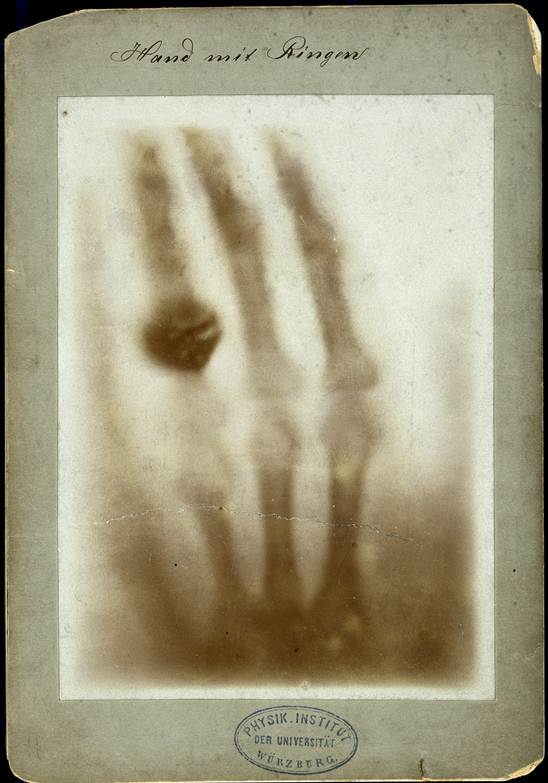
\includegraphics[height=6cm]{Images/first_CT.png}
    \adjincludegraphics[height=6cm,trim={{.15\width} {.10\height} {.15\width} {.10\height}},clip]{Images/Liver_ultrasound.jpg}
    \caption{Exemples d'acquisitions 2D. À gauche, la première image obtenue par rayons X (Roentgen, 1895). À droite, image par ultrason du foie \protect\footnotemark. La veine porte est visible en noir.}
    \label{fig:2D imaging}
\end{figure}

Ces méthodes, à l'origine limitées à la 2D, ne permettaient pas d'avoir un rendu des organes en trois dimensions. Deux techniques, communément employées aujourd'hui ont donc été développées pour acquérir des images volumiques 3D par empilement successif de coupes 2D.
\subsection{Tomodensitométrie}
\label{sec:contexte:images:CT}
La tomodensitométrie (TDM) est un système reposant sur l'émission de rayons X développée en 1979 par Hounsfield et al. \cite{Hounsfield1995_CT_machine}.\footnotetext{Source : \url{https://www.rcemlearning.co.uk/reference/ultrasound-in-emergency-medicine-level-1-instruction/\#1571742949461-1d2bb2b5-ad61}}

Le patient est allongé sur une table autour de laquelle est positionné un anneau. La table sur laquelle repose le patient est déplacée dans l'axe des pieds à la tête (axe longitudinal). L'anneau de la machine tomodensitométrique contient un tube émetteur de rayons X ainsi qu'une rangée de détecteurs sur la partie opposée de l'anneau. L'anneau tourne autour du patient afin d'acquérir le plan XY, ou plan axial. Pour les acquisitions avec une table immobile, on parle de mode axial ou séquentiel. Lorsque la table est en mouvement pendant l'acquisition, on parle de mode spiralé ou hélicoïdal. Cette technologie est irradiante, car une image est obtenue grâce à l'absorption du rayonnement par les organes qui atténuent de fait le signal reçu par les capteurs.  Une exposition à un rayonnement important peut être à l'origine de cancer, c'est pourquoi les doses auxquelles sont exposés les patients sont très contrôlées par les radiologues.

Les images produites par un système de TDM sont des sinogrammes, un type d'images qui contient la projection du profil détecté pour un certain angle du capteur. Chaque ligne du sinogramme représente ainsi la projection pour un angle donné. On peut ensuite reconstituer une image 2D grâce à la transformée de Radon (plus précisément son inverse), qui permet de reconstituer un point dans l'espace à partir de la totalité de ses projections. L'ensemble du processus est illustré en Fig. \ref{fig:tomography}.
\begin{figure}
    \centering
    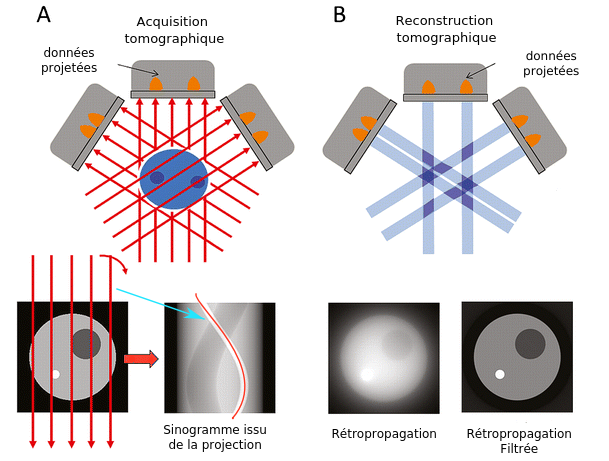
\includegraphics[height=8cm]{Images/Tomo_projection_2.png}
    \caption{Acquisition par projection et reconstruction du signal. En théorie l'image initiale est reconstruite grâce à un nombre infini de projections. En pratique, la reconstruction est finie, et donc incomplète, ce qui peut provoquer des artefacts de flou.}
    \label{fig:tomography}
\end{figure}
\subsubsection{Encodage des intensités}
Les intensités des images tomodensitométriques sont encodées dans une unité particulière, l'unité Hounsfield (HU). Cette unité mesure le coefficient d'atténuation du rayonnement. Elle fixe à 0 l'atténuation de l'eau distillée et à $-1000$ l'atténuation de l'air. La limite haute dépend du nombre de bits utilisés pour l'encodage des pixels de l'image ($\sim 3070$ HU pour l'acier en 12 bits vs. $\sim 13590$ HU en 16 bits) \cite{Glide2013_metal_saturation}. La gamme élevée de niveaux de gris des images TDM n'est pas détectable dans son ensemble par l'oeil humain et nécessite l'utilisation de fenêtres d'intensités ajustables dynamiquement.
\subsubsection{Artefacts des images tomodensitométriques}
Les artefacts liés à la tomodensitométrie sont multiples. Premièrement, la qualité de l'image dépend du nombre de projections disponibles. Les structures peuvent être floues du fait de la reconstruction. En effet, en théorie, une image nette est obtenue par la reconstruction d'un nombre infini de projections. En pratique le nombre de projections est défini et choisi comme un compromis entre rapidité d'acquisition et qualité de l'image. Le flou peut avoir d'autres causes telles que les mouvements du patient, la distance à la source, où être causé par l'absorption des tissus. 
\begin{figure}
    \centering
    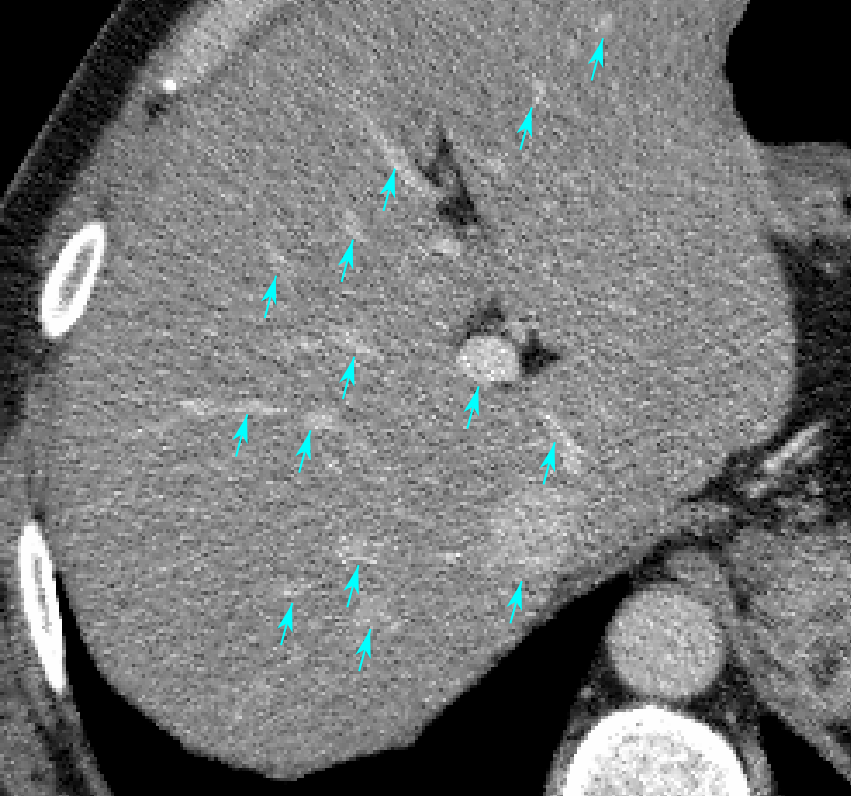
\includegraphics[height=8cm]{Images/blury_vessels_arrow.png}
    \caption{Coupe d'une tomographie du foie. Les structures claires aux bords flous  correspondent aux vaisseaux hépatiques (flèches).}
    \label{fig:CT_blur}
\end{figure}

Deuxièmement, les images tomodensitométriques présentent toutes un profil bruité (Fig. \ref{fig:CT_noise}). Ce bruit provient de la source de photons qui les émet de manière aléatoire. En théorie ce phénomène suit une loi de probabilité de Poisson. Cependant, le bruit affectant les images à la fin du processus est un bruit additif blanc gaussien \cite{Lei1992_gaussianNoiseCT}. Ce bruit est défini par la densité de probabilité suivante :
\begin{equation}
G(x) = \frac{1}{\pi \sqrt{2\pi} } \exp\big( \frac{ (x-\mu)^2}{2\sigma^2} )    
\end{equation}
Cette densité est paramétrée par la moyenne du bruit $\mu$ et son écart-type $\sigma$ qui correspond à la dispersion des valeurs d'intensité du bruit autour de sa moyenne.
\begin{figure}
    \centering
    \adjincludegraphics[height=8cm,trim={{0.3\width} {0.3\height} {0.3\width} {0.3\height}},clip]{Images/noise_CT.png}
    \caption{Visualisation du bruit gaussien sur une image du foie. Celui-ci produit une texture sablonneuse.}
    \label{fig:CT_noise}
\end{figure}

Enfin, ce type d'imagerie est sensible à une troisième catégorie d'artefacts liés aux objets métalliques tels que les broches. Ces objets provoquent des phénomènes de saturation sous formes de rayons concentriques observables en Fig. \ref{fig:metallic artefacts}.
\begin{figure}
    \centering
    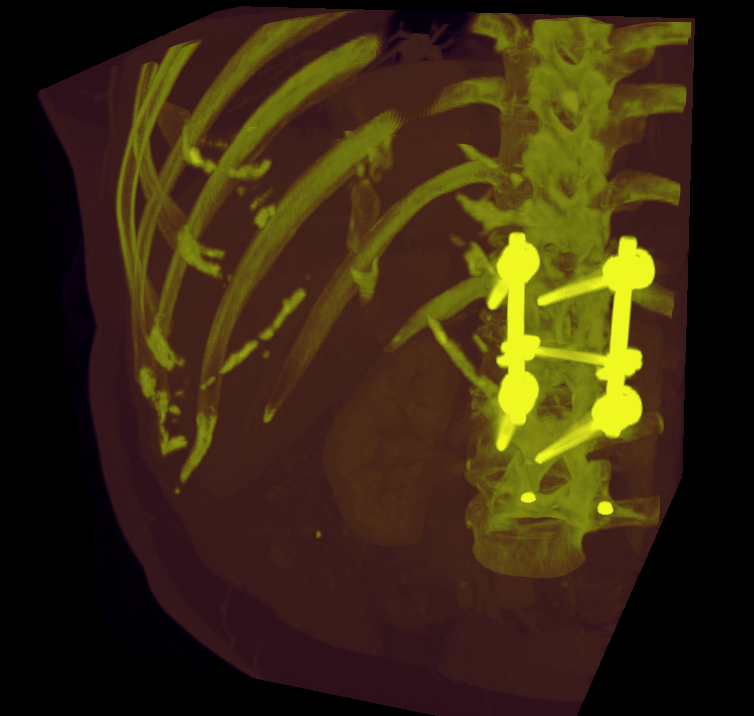
\includegraphics[height=6cm]{Images/broaches_CT.png}
    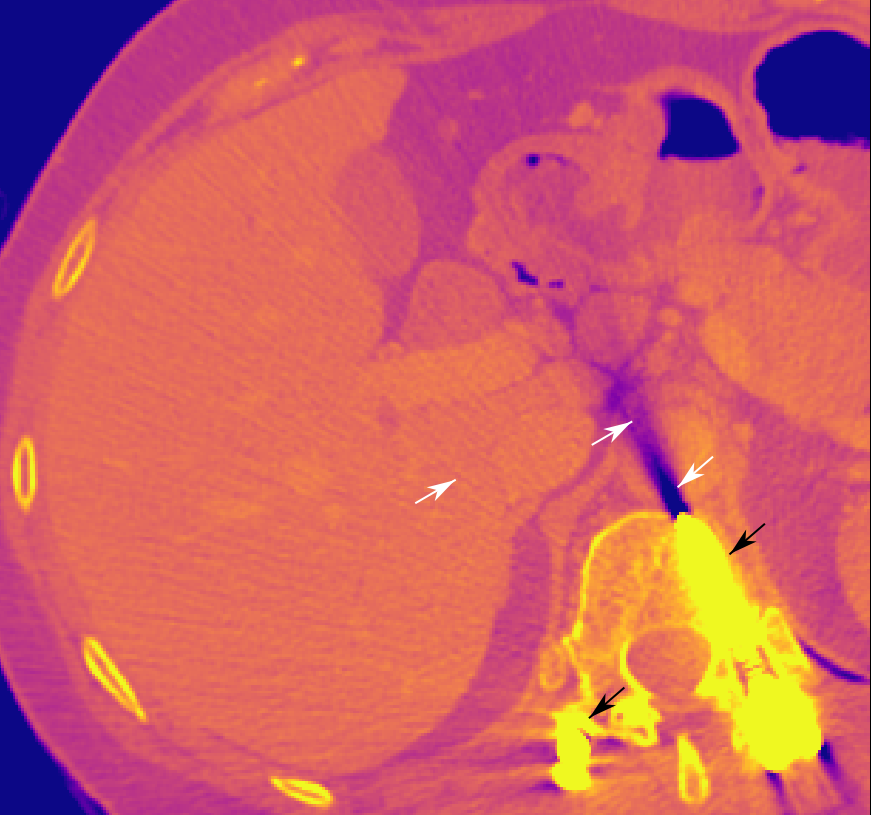
\includegraphics[height=6cm]{Images/broaches_CT_slice_arrow.png}
    \caption{Les broches métalliques, visibles dans la vue 3D (à gauche), provoquent des artefacts de saturation (flèches noires) et de rayonnement (flèches blanches) visibles sur les vues en coupe (à droite).}
    \label{fig:metallic artefacts}
\end{figure}

\subsection{Imagerie par résonance magnétique}
\label{sec:contexte:images:irm}
Les premières images du corps humain obtenues par résonance magnétique (IRM) ont été réalisées par Damadian et al. en 1977 \cite{Damadian1977_NMRI}. Les machines utilisées pour l'imagerie par résonance magnétique sont similaires en apparence à la tomodensitométrie. Le patient est aussi allongé sur une table et est positionné à l'intérieur d'un anneau. Ici, l'anneau contient des aimants qui produisent des champs magnétiques.

L'IRM repose sur la mesure du retour à l'équilibre du moment magnétique de particules chargées. Lorsque certains atomes sont soumis à un champ magnétique, ceux-ci s'orientent dans la direction du champ magnétique. Dans un système IRM, un champ magnétique constant permet d'aligner les atomes d'hydrogène constitutifs des tissus dans une certaine direction appelée axe longitudinal. Ces particules sont en précession, c'est-à-dire qu'elles tournent sur elles-même autour de l'axe longitudinal comme une toupie qui se stabilise le long de son axe de rotation. Lors de l'acquisition, un deuxième champ magnétique orthogonal au premier champ magnétique provoque une résonance avec les atomes d'hydrogène qui sont contraints d'augmenter leur angle de précession. Ce champ magnétique est ensuite arrêté, ce qui provoque un retour à la normale de la précession des atomes d'hydrogène. C'est le temps que prend la précession pour se réaligner avec l'axe longitudinal, appelé temps de relaxation, qui est à la base de différentes mesures physiques permettant de produire différentes séquences d'images en IRM (Fig. \ref{fig:T1_MRI}).

Le temps de relaxation est dépendant de l'agitation moléculaire. Si l'agitation est très faible comme dans les tissus durs (os), \newV{ou très forte comme dans les liquides}, la relaxation est lente. Au contraire, une agitation modérée caractéristique des tissus mous produit une relaxation rapide.
\begin{figure}
    \centering
    \adjincludegraphics[height=5.5cm,trim={{.08\width} {.06\height} {.1\width} {.05\height}},clip]{Images/T1_in_phase.png}
    \adjincludegraphics[height=5.5cm,trim={{0.04\width} {0.05\height} {0.04\width} 0},clip]{Images/T1_out_phase.png}
    \caption{Volumes de la base CHAOS en phase T1-in (gauche) et T1-out (droite). La différence du temps d'écho entre l'émission et la réception du signal produit des contrastes différents.}
    \label{fig:T1_MRI}
\end{figure}
\subsubsection{Artefacts des images IRM}
Les images IRM sont affectées par de nombreux artefacts. Nous présentons ici les trois principaux.

\newV{Le protocole d'acquisition pour les patients peut être source d'artefacts. Un examen IRM dure environ 20 à 30 minutes. Il est demandé au patient de rester immobile durant l'acquisition et des acquisitions incluant des périodes d'apnée peuvent être nécessaires pour l'imagerie abdominale, dont l'imagerie du foie. Pour certains patients, cet exercice peut-être difficile voire douloureux à réaliser. Il est donc courant d'observer des artefacts liés au mouvement de la respiration dans les images IRM (Fig. \ref{fig:MRI_movement}). Ceux-ci sont visibles de deux manières : la présence d'un organe fantôme légèrement décalé par rapport à l'organe lui-même, ou la fusion des tissus d'organes adjacents. Deux organes peuvent aussi se superposer et une fusion des tissus peut être visible sur les images.}
\begin{figure}
    \centering
    \adjincludegraphics[height=6cm,trim={{0.04\width} {0.15\height} {0.01\width} {0.15\height}},clip]{Images/MRI_movements_arrow.png}
    \caption{Artefacts de mouvement visibles sur les bords du foie (flèches bleues). Ceux-ci forment une seconde bordure d'intensité moindre autour du foie. Les mouvements peuvent aussi faire fusionner des organes adjacents (flèches rouges).}
    \label{fig:MRI_movement}
\end{figure}

Du bruit est aussi présent dans les images IRM. Ce bruit est particulier puisqu'il s'agit d'un bruit ricien \cite{Gudbjartsson1995r_Rician_noise_MRI}. Ce bruit n'est pas additif comme le bruit gaussien, mais est dépendant du signal. Il s'exprime par la densité de probabilité suivante : 
\begin{equation}
    f(x | \upsilon, \sigma) = \frac{x}{\sigma^2} exp ( \frac{-(x^2 + \upsilon^2)}{2\sigma^2} ) I_0 (\frac{x\upsilon}{\sigma^2})
    \end{equation}
avec $I_0(z)$ la fonction de Bessel de première espèce et d'ordre 0, \newV{ avec $\upsilon$ la distance à l'origine de la distribution et $\sigma$ son écart-type.}

la fonction de Bessel de première espèce d'ordre $n$ est une fonction à oscillation décroissante définie par :
\begin{equation}
I_n(x) = \frac{1}{\pi}\int_0^{\pi} \cos(nt - x\sin t) dt
\end{equation}
\newV{Lorsque le rapport signal sur bruit (SNR) est fort, la densité de probabilité de ce type de bruit approxime une distribution gaussienne \cite{Gudbjartsson1995r_Rician_noise_MRI}. Cependant, lorsque le SNR est faible, la distribution du bruit ne suit plus une distribution normale. Comme pour un bruit gaussien, le paramètre $\sigma$ contrôle l'étalement de la distribution du bruit (Fig. \ref{fig:MRI_Rice}).}
\begin{figure}
    \centering
    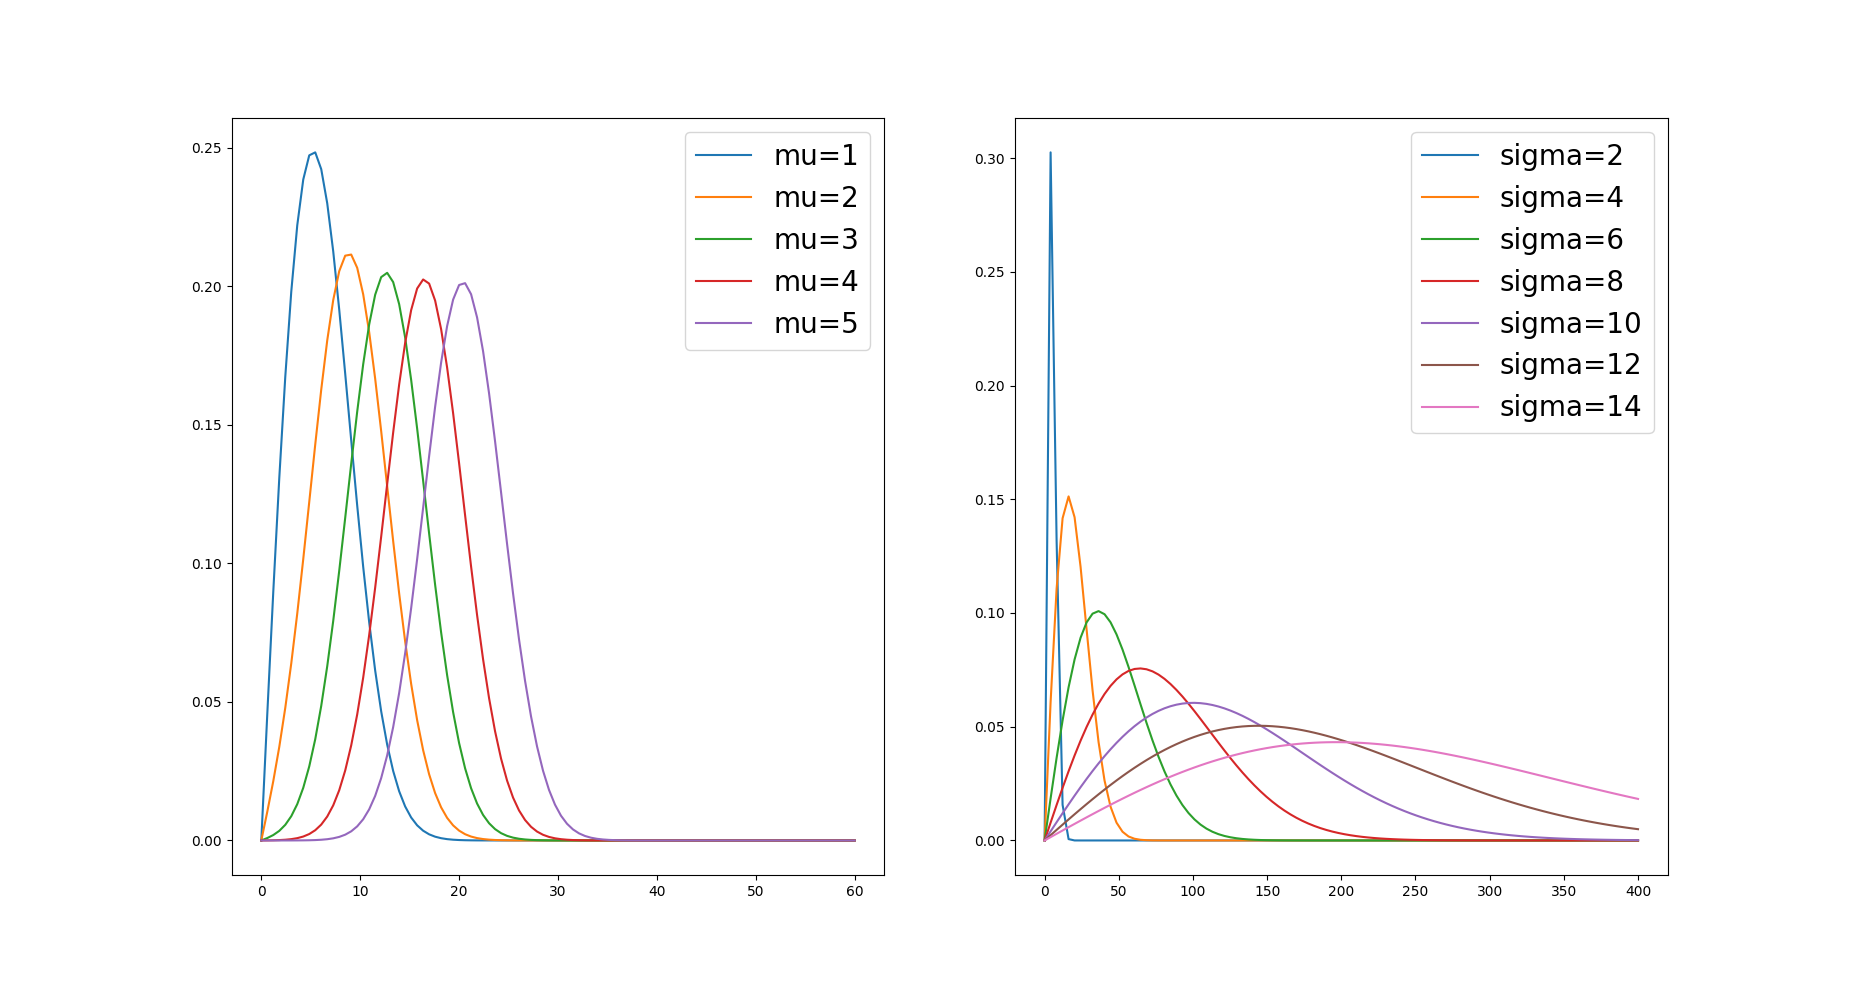
\includegraphics[width=\textwidth]{Images/noise_CT_2.png}
    \caption{Distributions de Rice. \newV{Au fur et à mesure que la distance à l'origine $\upsilon$ augmente la distribution de Rice approxime une distribution gaussienne (à gauche). $\sigma$ contrôle l'étalement de la courbe (à droite).}}
    \label{fig:MRI_Rice}
\end{figure}

Le positionnement de l'antenne par rapport au corps du patient peut aussi entrainer des variations dans le champ magnétique qui provoquent des variations d'intensité locales dans des zones homogènes. Ainsi, des tissus de même nature peuvent présenter des profils d'intensité variés (Fig. \ref{fig:MRI_variations}). Cet artefact complexifie certaines hypothèses lors du traitement des images IRM.
\begin{figure}
    \centering
    \adjincludegraphics[height=8cm,trim={{0.08\width} {0.05\height} {0.05\width} {0.05\height}},clip]{Images/MRI_field_variations.png}
    \caption{IRM du foie, T1-in. On observe une variation d'intensité pour des tissus de même nature. Le centre du foie est relativement plus sombre que les tissus sur ses bords alors qu'ils sont de même nature.}
    \label{fig:MRI_variations}
\end{figure}
\section{Données}
L'accès aux données TDM et IRM pour le contexte de la recherche  peut-être difficile. La législation sur la protection des données personnelles complexifie l'accès aux données des patients. En effet, la campagne de collecte de données dans un hôpital est soumise à un accord préalable d'un comité éthique puis l'accord des patients. Les données qui sont transmises aux chercheurs doivent être anonymisées, c'est-à-dire que les informations contenues dans les images telles que le nom du patient, le nom de la série ainsi que la date de l'acquisition doivent être effacés. Depuis la  directive européenne RGPD (Réglement Général sur la Protection des Données) le patient a la possibilité de rétracter son avis à tout moment, ce qui nécessite une politique d'anonymisation qui permette la tracabilité et la suppression des données. Par exemple, l'une d'entre elles est la \textit{tokenization}, qui permet d'attribuer une signature chiffrée à un volume.

\newV{Une fois les procédures éthiques et administratives validées, il est nécessaire d'annoter les données médicales.} Cela nécessite la supervision d'un médecin expert, car les organes à annoter sont complexes à identifier. \newV{Pour les vaisseaux sanguins, plusieurs types d'annotations sont possibles. On peut choisir d'annoter un vaisseau à partir d'une série de coordonées/points le long de son centre. La courbe passant par ces points est alors appelée ligne centrale.} Cette méthode est économe en temps d'annotations, mais ne fournit généralement pas d'informations précises sur l'aspect des vaisseaux et leur diamètre. 
Une autre méthode consiste à créer un masque de segmentation en annotant tous les voxels appartenant aux vaisseaux. Cette méthode est la plus complète, mais nécessite bien plus de temps à l'annotateur. De plus, la notion de frontière entre les structures peut varier d'un avis d'expert à l'autre. \newV{Bien que ce problème existe aussi pour la ligne centrale, il est plus marqué pour la segmentation voxélique dont les applications nécessitent une plus grande précision (i.e. détection d'anévrisme, connectivité des vaisseaux adjacents, etc.)}. Une solution possible consiste à moyenner le résultat parmi plusieurs annotateurs. Cette méthode demande cependant une mobilisation d'un nombre important de médecins. Il faut en effet garder à l'esprit que dans un hôpital, un médecin peut rarement consacrer du temps pour annoter des données, ce qui rend ce type d'initiatives rare. Les deux types d'annotations sont illustrés en figure \ref{fig:annotations}. 
\begin{figure}
    \adjincludegraphics[width=0.45\textwidth,trim={{0.5\width} {0.3\height} {0.0\width} {0.2\height}},clip]{Images/vessels_centerline.png}
    \adjincludegraphics[width=0.45\textwidth,trim={{0.5\width} {0.3\height} {0.0\width} {0.2\height}},clip]{Images/vessels_segmentation.png}
    \caption{Annotations d'un vaisseau : ligne centrale (à gauche) vs. masque de segmentation (à droite). L'annotation de la ligne centrale est bien moins coûteuse en temps d'annotations car elle nécessite seulement de poser un nombre limité de points de contrôle. Le masque de segmentation capture quant à lui l'entièreté du vaisseau.}
    \label{fig:annotations}
\end{figure}

\newV{Face à ces difficultés administratives et techniques, une grande partie des bases des données utilisées dans les résultats de publications sont privées. Les auteurs citent en général les conditions d'acquisition et le nombre de volumes disponibles, mais ne donnent pas d'accès aux données. Certains jeux de données sont tout de même disponibles publiquement.}

\newV{Dans le cadre du projet ANR, une collecte de données a été réalisée. Cependant, le processus administratif a débuté en même temps que cette thèse. Il a donc fallu se tourner vers des données publiques ne nécessitant pas de procédures d'accès. Un aspect positif de cette contrainte est que l'utilisation de données publiques a renforcé la reproductibilité et la  réutilisation de nos travaux.}

\newV{Afin d'étudier les filtres de rehaussement de vaisseaux dans le contexte de l'imagerie du foie, nous avons recensé les différentes bases de données hépatiques disponibles en ligne. Afin de réaliser une analyse complète du rehaussement pour le foie, nous avons cherché des bases de données de modalité TDM et IRM.}
\newV{Nous passons ici en revue les jeux de données publics pour l'organe du foie et discutons des avantages et limites de chacun. Nous présentons ensuite deux jeux de données alternatifs qui nous ont permis de compléter notre analyse.}
\subsection{Ircad}
La base de donnée 3DIrcadb1 \cite{Soler20103_ircad} est proposée par l'Institut de recherche contre les cancers de l'appareil digestif (Ircad) de Strasbourg. Cette base contient des images de tomodensitométrie de l'abdomen (Fig. \ref{fig:Ircad_examples}). Elle contient les images de 20 patients répartis en 50 \percent{}homme/femme et 75 \percent{}de foies lésés. Pour chaque patient une image tomographique inclut le foie et mesure entre $512 \times 512 \times 74$ et $512 \times 512 \times 260$ voxels pour une résolution des coupes axiales variant entre 0.56 mm et 0.87 mm et une épaisseur des coupes variant entre 1.00 mm et 4.00 mm. Elle fournit aussi un masque voxélique des organes de l'abdomen. Pour le foie, les masques des deux systèmes veineux porte et hépatique (incluant la veine cave) sont fournis dans des volumes différents. Un masque des tumeurs du foie est également disponible.
\begin{figure}
    \centering
    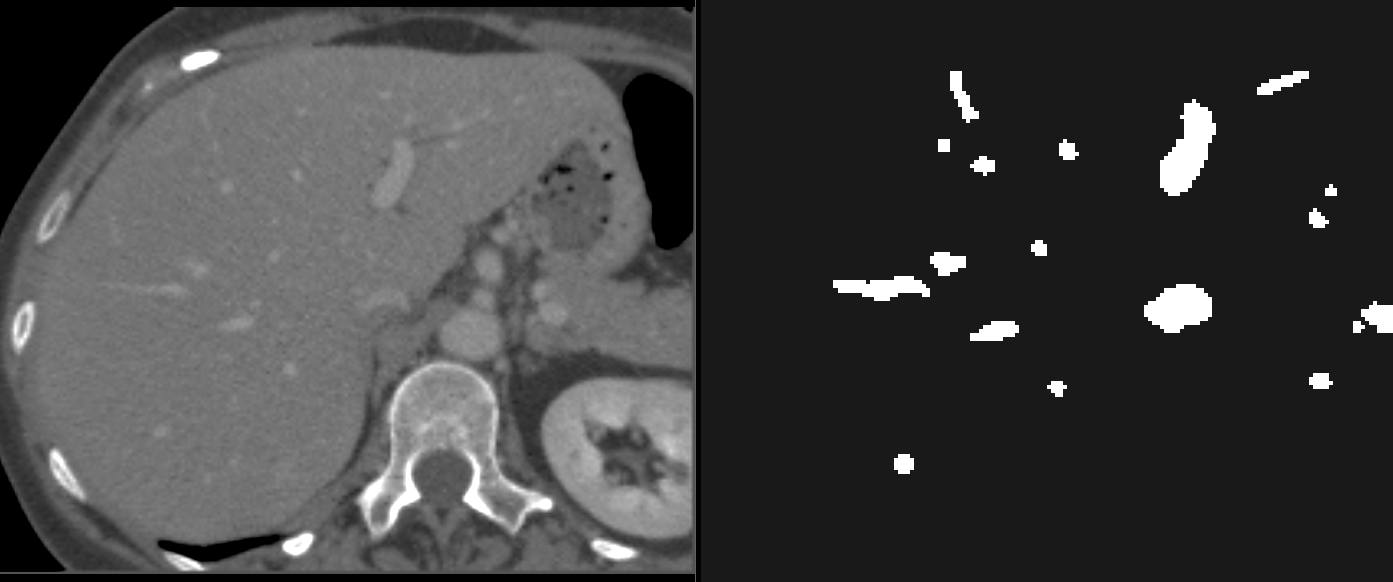
\includegraphics[height=6cm]{Images/Ircad_examples.png}
    \caption{À gauche, coupe du foie issue d'un volume de l'Ircad. À droite, vérité terrain des vaisseaux. La vérité terrain est conçue comme un masque binaire.}
    \label{fig:Ircad_examples}
\end{figure}

Cette base datant de 2010 est la base la plus complète pour la segmentation des vaisseaux du foie. Cependant, elle n'est pas exempte d'anomalies. 

Premièrement, le nom des vérités terrain n'est pas consistant et indique sans doute que deux médecins différents ont participé à l'annotation des données. Deuxièmement, le volume du masque du foie contient des voxels parasites qui produisent de petites composantes connexes déconnectées du masque. Elles interfèrent avec les traitements sur les masques comme la sélection de la boîte englobante du foie.
 Enfin, certains vaisseaux à l'intérieur du foie ne sont pas annotés, ce qui représente un problème crucial. Cela concerne des petites structures tubulaires mesurant quelques voxels de large, mais aussi de gros vaisseaux (Fig. \ref{fig:missing_annotations}). Ces oublis perturbent forcément l'évaluation des méthodes de segmentation puisque des vaisseaux non annotés pourraient tout de même être détectés et comptés comme des segmentations erronées. 

Ce biais est difficile à quantifier dans la mesure où il faudrait compléter manuellement la segmentation pour se rendre compte de son impact réel. Celui-ci est toutefois à garder à l'esprit pour la comparaison de filtres dont les performances sont très différentes dans une zone d'intérêt spécifique.
\begin{figure}
    \centering
    \adjincludegraphics[height=8cm,trim={{0.02\width} {0.15\height} {.02\width} {0.12\height}},clip]{Images/missing_annotations.png}
    \caption{Vue 3D du foie. En vert, vérité terrain des vaisseaux. Des vaisseaux très visibles en 3D ne sont pas inclus dans la vérité terrain.}
    \label{fig:missing_annotations}
\end{figure}
\subsection{CHAOS}
Le jeu de donnée CHAOS est issu du challenge \cite{CHAOS2021} du même nom (CHAOS challenge - Combined (CT-MR) Healthy Abdominal Organ Segmentation). Celui-ci propose deux jeux de données avec deux modalités différentes. Un premier jeu contient 40 images TDM obtenues après injection d'agent de contraste dans la veine porte. L'acquisition est prise 70 à 80 secondes après l'injection et elle permet de mettre en valeur le système veineux porte et une partie de la veine hépatique. Ce jeu de données possède des coupes d'images de résolution $512\times 512$ voxels avec une résolution entre 0.7 mm et 0.8 mm dans le plan XY et 3 mm à 3.2 mm dans l'axe Z.

Un second jeu IRM inclut 120 volumes acquis selon des méthodes différentes : 40 volumes acquis en phase T1-in (Fig. \ref{fig:T1_MRI_2}), 40 volumes  en phase T1-out (Fig. \ref{fig:T1_MRI_2}) et 40 séquences en phase T2 spiralée (Fig. \ref{fig:T2_MRI}). La pondération de contraste T2 rend les vaisseaux du foie hyper-intense et l'acquisition spiralée permet de mieux séparer les tissus tout en limitant les artefacts de mouvement.
\begin{figure}
    \centering
    \adjincludegraphics[height=5.5cm,trim={{.08\width} {.06\height} {.1\width} {.05\height}},clip]{Images/T1_in_phase.png}
    \adjincludegraphics[height=5.5cm,trim={{0.04\width} {0.05\height} {0.04\width} 0},clip]{Images/T1_out_phase.png}
    \caption{\newV{Volumes de la base CHAOS en phase T1-in (gauche) et T1-out (droite). On peut observer une différence de contraste provoquée par un temps d'écho différent, i.e. le temps entre l'émission et la réception du signal.}}
    \label{fig:T1_MRI_2}
\end{figure}

Ce jeu de données est intéressant dans le sens où il propose plusieurs types de modalités IRM. Contrairement à l'Ircad, la résolution dans l'axe Z est plus élevée (Fig. \ref{fig:CHAOS_geometry}), ce qui tend à indiquer que la base a été acquise en vue de traitements coupe par coupe plutôt que volumique. En effet, la représentation 3D des vaisseaux est grandement dégradée par ce type d'acquisition.  De plus, l'objectif de cette base étant la segmentation des organes abdominaux, elle ne propose que le masque du foie comme annotation.
\begin{figure}
    \centering
    \adjincludegraphics[height=6cm,trim={{0\width} {0.08\height} {0.02\width} {0\height}},clip]{Images/T2_SPIR.png}
    \caption{Volume de la base CHAOS acquis en phase T2 spiralée. Le contraste des vaisseaux est plus important en pondération T2.}
    \label{fig:T2_MRI}
\end{figure}
\begin{figure}
    \centering
    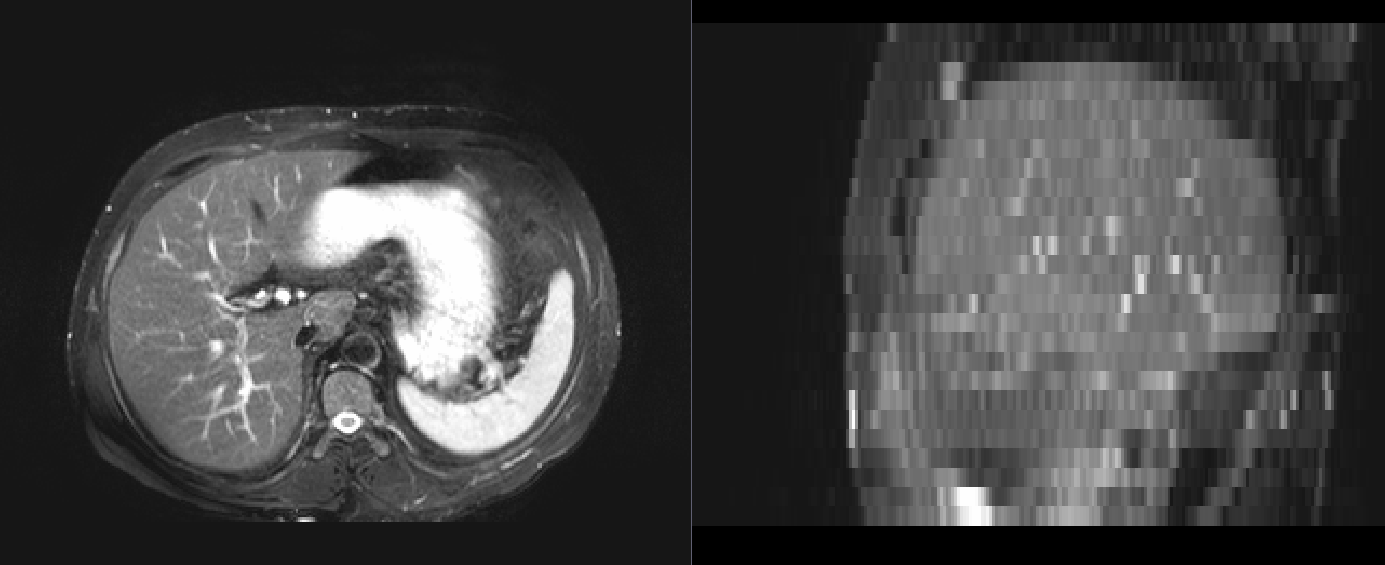
\includegraphics[width=\textwidth]{Images/CHAOS_resolution.png}
    \caption{Volume de la base CHAOS en phase T2 spiralée. Comparaison de la résolution axiale (gauche) et sagittale (droite). Dans la vue sagittale la géométrie des structures, en particulier les vaisseaux, est largement altérée.}
    \label{fig:CHAOS_geometry}
\end{figure}
\subsection{Medical Decathlon}
Le challenge Medical Decathlon \cite{antonelli2022medical} propose de mesurer les performances d'algorithmes de segmentation sur 10 tâches qui regroupent différents organes (cerveau, cœur, hippocampe, foie, pancréas, prostate, colon, rate). Le challenge regroupe un nombre significatif de volumes par tâche, de 30 volumes pour le cœur jusqu'à 750 volumes pour le cerveau. Une modalité par organe est proposée : IRM pour le cerveau, le cœur, l'hippocampe, la prostate et la tomodensitométrie pour les autres organes. Deux tâches concernent le foie, toutes deux acquises en phase veineuse porte. La première tâche concernant la segmentation du foie et des tumeurs hépatiques contient 210 volumes. La seconde tâche concernant la segmentation des vaisseaux et des tumeurs hépatiques regroupe 443 volumes.

Les données hépatiques pour la première tâche ont été sélectionnées pour leur variabilité en termes de taille de labels avec de fortes variations de taille de foie, de nombre de tumeurs, etc. Ces données ont été acquises au centre de l'Ircad de Strasbourg. La résolution des images pour cette tâche est de 0.5 mm à 1.0 mm dans l'axe XY et 0.45 mm à 6.0 mm dans l'axe Z. Les annotations sont réalisées par un expert radiologue.

Les données hépatiques pour la seconde tâche (Fig. \ref{fig:MD_examples}) sont issues de patients présentant des tumeurs hépatiques parfois métastasées. Les vaisseaux sanguins présentent parfois des connexions au niveau des tumeurs. Ces données ont été acquises par le centre contre le cancer Memorial Sloan à New York. Pour cette tâche, la résolution des images dans l'axe Z varie de 2.5 mm à 5.0 mm. Les masques de segmentation ont été annotés de manière semi-automatique au moyen d'une approche par croissance de région. Les contours ont ensuite été ajustés par des radiologues.

Cette base de données a l'avantage de proposer un grand nombre de volumes dans plusieurs modalités. Cependant, l'annotation semi-automatique produit une vérité terrain moins précise, en particulier pour les petits vaisseaux. On peut aussi noter un nombre conséquent de vaisseaux déconnectés du réseau vasculaire dans les annotations. De plus, pour le foie, une résolution supérieure à 3 mm, comme illustré dans CHAOS (Fig. \ref{fig:CHAOS_geometry}), dégrade fortement la géométrie des vaisseaux sur laquelle se basent les filtres de rehaussement 3D.
\begin{figure}
    \centering
    \adjincludegraphics[width=\textwidth,trim={{0\width} {0.2\height} {0\width} {0.02\height}},clip]{Images/MD_examples.png}
    \caption{Challenge Medical Decathlon. Volume hépatique en TDM (gauche) et la vérité terrain associée (droite).}
    \label{fig:MD_examples}
\end{figure}
\subsection{Données synthétiques : VascuSynth}
Lorsque des données cliniques munies d'annotations sont difficiles à obtenir, une autre solution est de générer un volume contenant un réseau vasculaire synthétique. VascuSynth \cite{Hamarneh2010_vascuSynth} est un programme permettant de créer un réseau vasculaire en fonction d'une carte d'oxygénation et des paramètres de pression sanguine à l'entrée de celui-ci. Le réseau vasculaire est construit de manière itérative de sa racine jusqu'aux extrémités. L'utilisateur peut de plus paramétrer la complexité du réseau en spécifiant le nombre de bifurcations attendu. Il est aussi possible d'ajouter du bruit additif gaussien au volume.

La résolution est \newV{isométrique} pour l'ensemble des axes. Les vaisseaux de VascuSynth présentent des profils d'intensité quasi homogènes, avec une intensité des voxels moindre près des parois. Les volumes ont un fond nul. La vérité terrain des vaisseaux, précise au voxel près, peut donc être obtenue par simple seuillage.

Une base de données pré-générée est disponible sur le site de VascuSynth. Celle-ci propose 120 volumes répartis en 10 groupes de 12 volumes. Chaque groupe contient des volumes de réseaux vasculaires dont le nombre de bifurcations varie entre 1 et 56 avec un pas de 5 (1, 6, 11, ..., 56) comme illustré en Fig. \ref{fig:VascuSynth}. Le jeu de données est aussi fourni avec un fichier Matlab contenant les coordonnées des bifurcations.

Les bases de données synthétiques possèdent les vérités terrain les plus complètes. Cependant, le contexte de ces jeux de données est beaucoup plus simple que les images réelles. Il est en effet difficile de simuler de manière réaliste des organes vascularisés dont les conditions de développement sont multifactorielles et qui dépendent à la fois de mécanismes génétiques et aléatoires qui sont compris seulement en partie. Les vaisseaux générés sont ainsi plus simples, dans le cas de VascuSynth : les vaisseaux sont des tubes pleins droits et discrétisés.
\begin{figure}
    \centering
    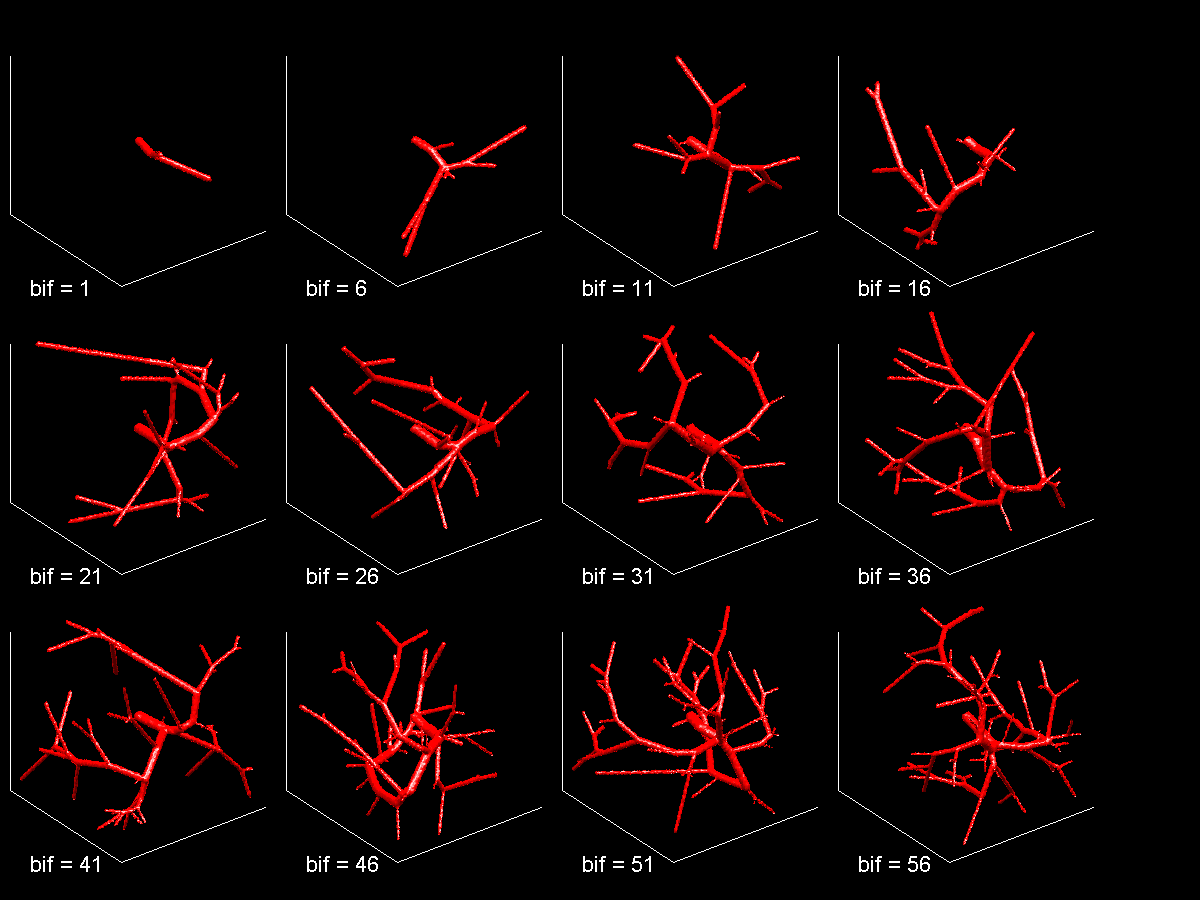
\includegraphics[height=8cm]{Images/snapVascu.png}
    \caption{Exemples de volumes issus de la base VascuSynth\_2013.}
    \label{fig:VascuSynth}
\end{figure}
\subsection{Bullitt}
\newV{Les bases de données IRM du foie sont limitées en termes de vérité terrain des vaisseaux. Lorsque des annotations des vaisseaux sont disponibles, la faible résolution des volumes ne permet pas une bonne analyse géométrique sur laquelle repose les filtres de rehaussement. Nous avons tout de même souhaité nous servir d'un jeu de données d'IRM réelles sans annoter nous-même une quantité importante de vaisseaux. Nous avons donc décidé d'élargir notre recherche de jeux de données à d'autres organes.}

\newV{Nous avons ainsi sélectionné le jeu d'images de cerveaux sains, Bullitt \cite{bullitt2005vessel}, comme jeu d'IRM réelles. Un soin particulier a été apporté à l'acquisition des images pour Bullitt qui présente un contraste remarquable entre les vaisseaux et le reste de l'image. Sur une partie de ces données (une trentaine de volumes), la ligne centrale et le rayon des vaisseaux sont fournis. Une segmentation des vaisseaux peut être reconstruite nativement grâce à l'outil tubeTK ; cependant la reconstruction est faite à partir d'un tube circulaire et a tendance à sous-estimer / omettre des voxels appartenant aux vaisseaux.}

Les travaux de Sanchesa et al. \cite{Sanchez2019_annotations_deep} améliorent ces vérités terrains de manière significative en augmentant de 70 \percent{} le nombre de voxels appartenant à la segmentation initiale, ce qui permet l'utilisation d'annotations plus précises (Fig.  \ref{fig:Bullitt_annotation_ameliorations}).
\begin{figure}
    \centering
    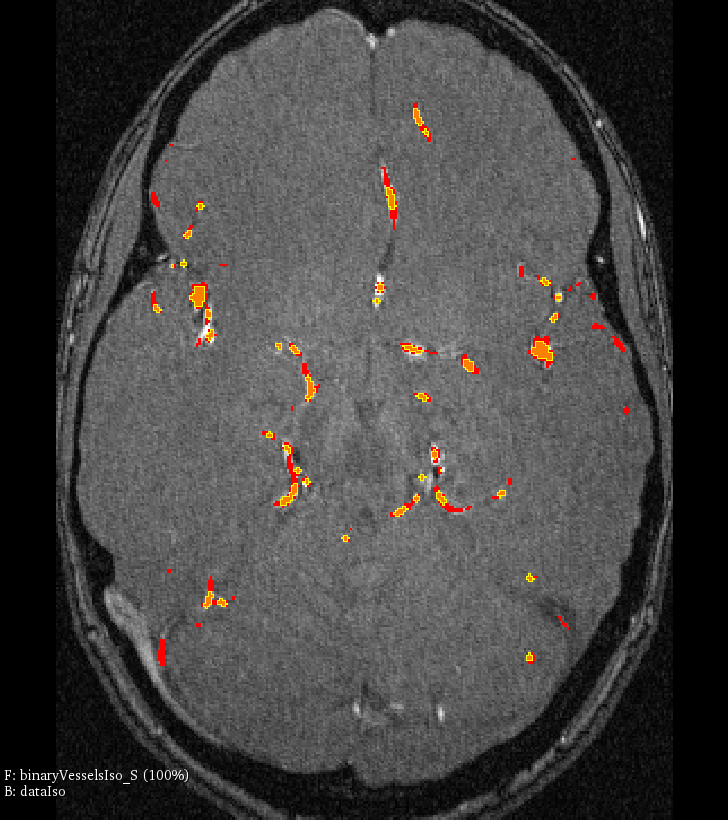
\includegraphics[height=6cm]{Images/Bullitt_annotation_ameliorations.png}
    \caption{Différence d'annotations entre reconstruction de la ligne centrale par tubeTK (jaune) et corrections d'annotations par Sanchez et al. (rouge). }
    \label{fig:Bullitt_annotation_ameliorations}
\end{figure}

Cette base de données est particulièrement bien acquise et présente très peu d'artefacts comparativement à des images IRM classiques. \newV{Les seuls artefacts notables sont un faible bruit constant sur l'ensemble de l'image et quelques coupes de contraste discontinues par rapport au reste de l'image. (Fig. \ref{fig:Bullitt_example}).}
\begin{figure}
    \centering
    \adjincludegraphics[height=6cm,trim={{0.02\width} {0.02\height} {0\width} {0.12\height}},clip]{Images/Bullitt_examples.png}
    \caption{Vue axiale et sagittale d'un volume issu de Bullitt. Les vaisseaux (structures blanches) sont particulièrement contrastés par rapport aux autres tissues adjacents.}
    \label{fig:Bullitt_example}
\end{figure}
\subsection{Bases de données relatives au projet R-Vessel-X}
Il était prévu pour le projet ANR une campagne de collecte de données TDM et IRM durant la durée du projet et commençant en même temps que la thèse. Cette collecte devait être réalisée sur des patients en cours de traitement. Cependant, la nécessité d'obtenir l' accord d'une commission éthique puis le besoin d'obtenir un espace de stockage dédié avec une société accréditée a retardé la collecte des données d'au moins un an. Celle-ci a finalement débouché sur une collecte de données rétrospective (patients ayant quitté l'hôpital) en même temps que le développement d'un logiciel d'annotation de données (Chap. \chapReproN{}). Ces données n'ont pas été exploitées dans nos travaux, puisqu’elles n’étaient pas prêtes au moment de notre étude.
\section{Bilan}
\label{sec:contexte:bilan}
Dans un premier temps, nous avons choisi d'utiliser deux jeux de données : la base de l'Ircad et le jeu de données de VascuSynth\_2013. La base de l'Ircad contient des artefacts variés de TDM (bruit, artefacts métalliques, etc.) et des masques de segmentation pour tous les volumes. Cela nous permet d'évaluer plus aisément les performances des algorithmes employés dans nos travaux. De plus, la résolution spatiale des volumes est l'une des meilleures parmi les bases disponibles. On peut ainsi utiliser des traitements 3D plutôt que de considérer un volume comme une séquence de coupes 2D. VascuSynth\_2013 offre une précision des vérités terrains qui n'est pas possible sur les bases réelles. C'est donc une base que nous avons jugée nécessaire pour notre travail. Celle-ci nécessite toutefois un traitement complémentaire afin de rendre les volumes proches d'une acquisition réelle. Ce traitement est décrit dans le chapitre 3 où nous avons choisi d'ajouter des artefacts IRM aux données.

\newV{Afin de compléter nos jeux de données et de diversifier nos expériences, nous avons choisi la base de données IRM, Bullitt, qui présente des vaisseaux fins dont la géométrie est naturelle comparée au jeu d'IRM synthétique. La qualité d'image de Bullitt, qui rend trivial le filtrage des vaisseaux, n'est cependant pas représentative des images IRM acquises habituellement. Nous avons donc dégradé ces images par un processus expliqué dans le chapitre \chapBenchN{}.}

Les spécificités des trois bases de données sont récapitulées dans la table \ref{tab:db_for_exp}. Comme nous le verrons dans le chapitre 3, ces bases de données requièrent des traitements complémentaires, avec notamment l'ajout de vérités terrain supplémentaires. Ces modifications sont nécessaires afin de proposer une analyse détaillée du rehaussement de vaisseaux que nous allons présenter dans le chapitre suivant.
\begin{table}[!ht]
    \caption{Jeux de données retenus pour la suite de nos travaux. Ces jeux de données sont complémentaires, au niveau des modalités utilisées, de la variété des organes étudiés ou de la précision des vérités terrains.}
    \label{tab:db_for_exp}
    \resizebox{\textwidth}{!}{
    \centering
    \begin{tabular}{ l|c|c|c|c }
        \hline
        Jeux de données & Modalité & Organe & Dimensions & Résolution \\
        \hline
        \multirow{2}{*}{Ircad}           & \multirow{2}{*}{TDM} & \multirow{2}{*}{Foie} & entre $512 \times 512 \times 74$  & $XY \in [0.56,0.87]$ mm   \\
                        &     &      & et $512 \times 512 \times 260$ voxels & $Z \in [1.00,4.00]$ mm \\
        \hline
        \multirow{2}{*}{VascuSynth}      & Synthétique / & \multirow{2}{*}{Aucun} & \multirow{2}{*}{$128 \times 128 \times 128$ voxels} & \multirow{2}{*}{$1\times1\times1$ mm} \\
                        & IRM simulée   &       &                                    &          \\
        \hline
        Bullitt         & IRM + artefacts ajoutés & Cerveau & $128 \times 448 \times 448$ voxels  & $0.5 \times 0.5 \times 0.8$  mm \\
        \hline
    \end{tabular}
    }

  \end{table}


